\chapter{Visualization for Explainable Classifiers}\label{sec-visualization}

As discussed at the end of \autoref{sec-explainable-classifier}, current research only focuses on one subject of the problem of explainable classifier and neglects the other subject -- human. Thus, we study explainable classifier from the aspects of visualization and human computer interaction in this chapter. Broadly speaking, the visualization for explainable classifiers can be viewed as a special case of algorithm visualization or software visualization. The former aims to provide better understanding of algorithms for education purposes in computer science. The latter focus on assisting developers and operation engineers for the development and maintenance of complex software. Here, the subject of visualization is the classifiers, which can be treated as algorithms learned from the data, or complex systems that need assistance in understanding.
% Unlike the previous chapter that discuss various algorithms for enhancing the explainability of classifiers,

We view the development and the operation of an intelligent system as a system engineering problem, and divide the life cycle of an intelligent system into different stages. The classification system can be treat as a specification of the general intelligent system. Then, we identify the current issues in explaining classifiers and discuss the research opportunities of visualization regarding different stages.

\section{Life Cycle of an intelligent system}

\begin{figure}[hb]
    \centering
    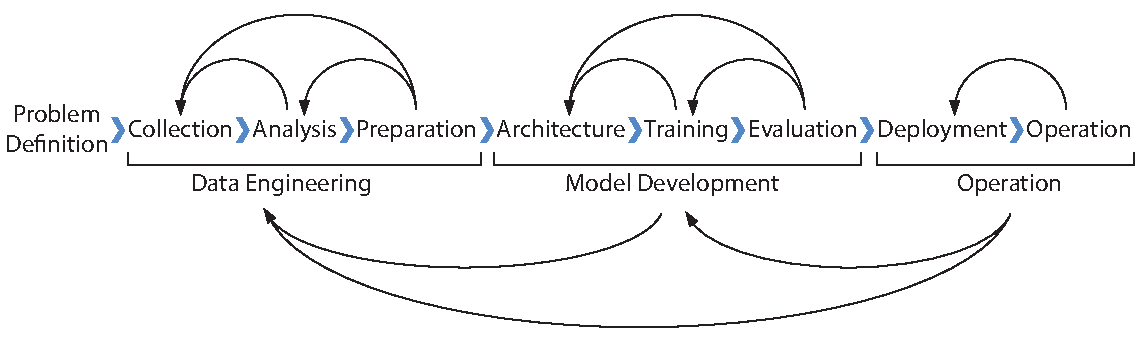
\includegraphics[width=1.0\textwidth]{figure/life-cycle}
    \caption{The life cycle of a classifier.}
    \label{fig:life-cycle}
\end{figure}

A classification system can be thought as a specialized case af an intelligence system. An intelligent system is developed to perform certain tasks with artificial intelligence (here we only consider data-driven systems). 
The development of a data-driven intelligent system is an iterative process. In this survey, the entire life cycle of an intelligent system is divided into three major stages (data engineering, model development, and operation) and eight sub-procedures (see \autoref{fig:life-cycle}). This definition is formed based on the cross-industry standard process for data mining \cite{wirth2000crisp}, a professional advice from Gartner, Inc. \cite{carlton2017ml}, the life cycle for expert system \cite{lasalle1990expert-system}, and the machine learning workflow of Google Cloud\footnote{\url{https://cloud.google.com/ml-engine/docs/ml-solutions-overview}}.

The first stage, data engineering, is defined to include any procedures that are data-related, namely, data collection, exploratory analysis, data preparation. The second stage, model development, includes procedures such as designing the architecture of the classifier (\eg, what type of model to use and parameters), training the model using data prepared, and evaluating whether the model meets certain requirements. After developing a classifier, the model is deployed, and in certain cases, is operated by some people. As we can see from \autoref{fig:life-cycle}, there are back-links from each stage/step to its previous stages/steps. This is the nature development. For example, we have a model with unsatisfactory performance after the training. This might due to model used is not suitable for certain tasks (go back to architecture setting), or it is because the volume of the data is too small (go back to collect more data). Similar problems might occur in other stages or procedures, which force us to go back and improve. 
%For example, if we are to develop a system for hospitals to detect early signs of lung cancer from a CT scan, the procedure goes as: 

Visualization and visual analytics systems are semi-automatic solutions at different stages to make a classifier more explainable. In the stage of data engineering, data visualization can help humans explore the data and get a qualitative sense of the nature of the data. Since the training of a classifier is actually extracting information from the training data, with more knowledge of the data in mind, humans (\ie developers or data scientists) can better understand if a failure results from the quality or volume issues of the data. At the second stage, visual analytics systems serve as development tools, which make the development more transparent and understandable. When designing or selecting model architectures, visual analytics systems can help humans better understand the characteristics of different classifiers, and even inspire improvements in the architecture. Visual diagnosing tools can help identify the problems in the training process and improve the debugging efficiency. For evaluations, visual analytics systems can help compare different classifiers and qualitatively evaluate the robustness and fairness of a classifier. At the last stage, when a classification system is deployed, visualization can help explain the inner workings of the system to end-users. For routine operations, visualization can better explain the predictions of the system, which make the monitoring and management easier. Also note that, visualization can used in the life-cycle for other purposes instead of explainability. For example, monitoring the training process by plotting loss curves, or visualization for crowd sourcing to collect data with better quality.

% -------

% A table summarizing all related papers

% -------

\section{Visualization for Exploratory Data Analysis}

In the stage of data engineering, visualization can be used mainly in the procedure of data analysis to assist humans' understanding of the data. Data plays an important role in the success of machine learning advances. A trained classifier can be viewed as a machine that has extracted the information in the training data and abstracted the information as its parameters. Different classifiers are suitable for datasets with different characteristics. Besides, a classifiers performance is largely depend on the quality of its training data. Thus, understand the data is the first step to understand a classifier.

There is a long history of research in visualization for exploratory data analysis. When comes to the classification problem, the data involved is \textbf{multi-dimensional data} with categorical labels, usually having the type of images, texts and categorical data. There are mainly three tasks: statistical analysis, dimensionality reduction, and dataset diagnostics.

\begin{figure}[hbt]
    \centering
    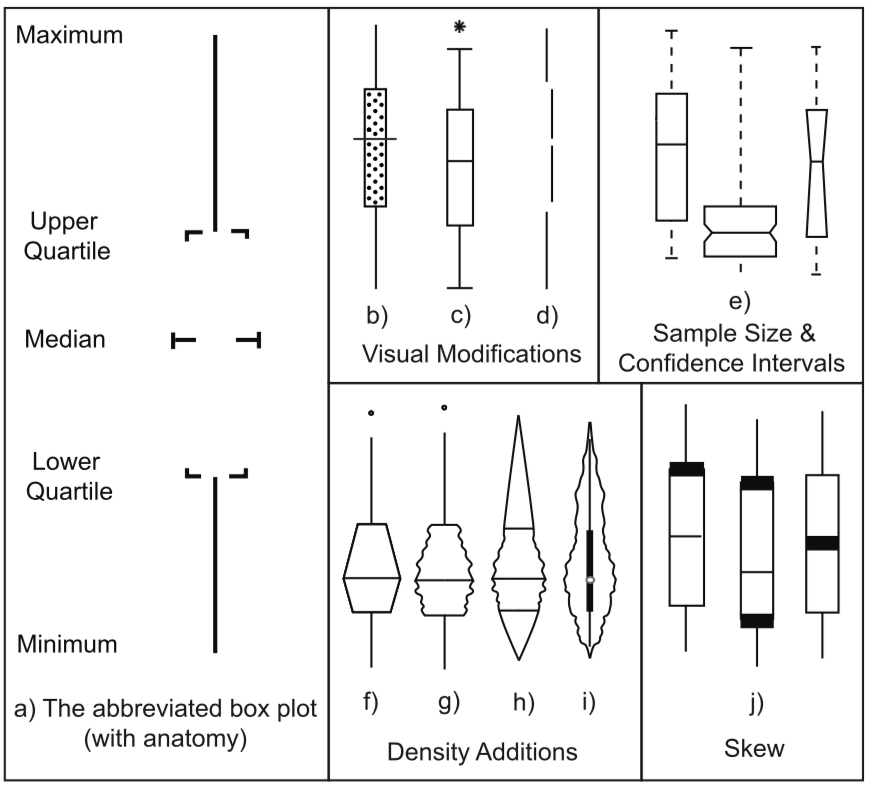
\includegraphics[width=0.7\textwidth]{figure/box-plots}
    \caption{Variations on the box plot \cite{potter2010statistics}. a) Abbreviated box plot. b) Range plot. c) Box plot. d) Interquartile plot. e) Variable width and notched box plots expressing sample sizes and confidence levels. f) Hist plot. g) Vase plot. h) Box-percentile plot. i) Violin plot. j) Skew and modality plots.}
    \label{fig:box-plots}
\end{figure}

\textbf{Statistical analysis}. The purpose of statistical analysis is to summarize statistical features of the datasets and provide users with a statistical understanding. One of the most influential visualization design is the box plot, which summarizes the key statistics of each feature in a box-like visualization. A survey on the design of box plots is provided by Potter \etal \cite{potter2010statistics}. As shown \autoref{fig:box-plots}, (a) presents the key features of a box plot. The box plots can be enhanced to embed more information such as confidence intervals in (e) and distribution densities in (f-i), providing more comprehensive summaries than the simple box plot. However, the datasets used in classification systems have become increasingly complex, with very high dimensions. Navigating through hundreds of box plots not necessarily provide insights about the datasets.

\begin{figure}[hbt]
    \centering
    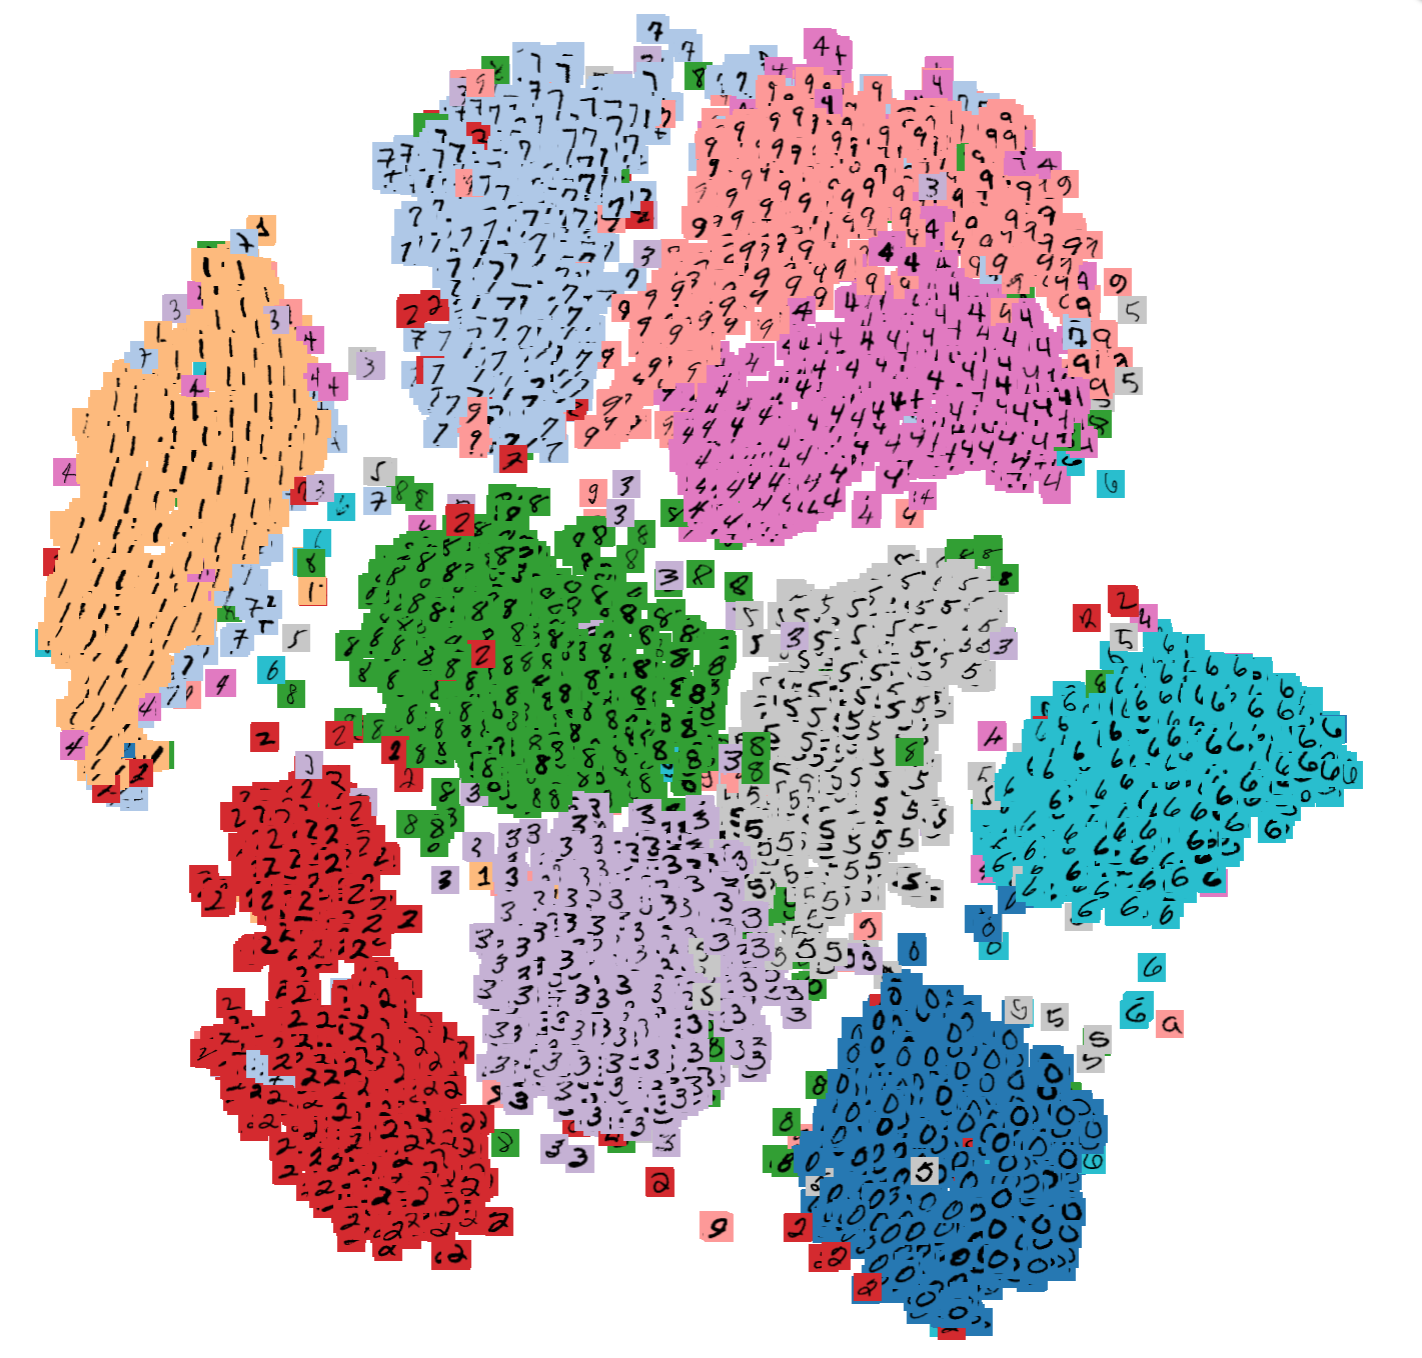
\includegraphics[width=0.7\textwidth]{figure/projector}
    \caption{The t-SNE projection of the MNIST dataset, colored by the labeled digits.}
    \label{fig:projector}
\end{figure}

\textbf{Dimensionality reduction}. In exploratory analysis, dimensionality reduction is usually applied for understanding how the data is distributed in the input space. Thus, projection, including principle component analysis (PCA), multidimensional scaling (MDS) \cite{kruskal1978mds}, and t-distributed stochastic neighbor embedding (t-SNE) \cite{maaten2008tsne}, is the most common dimensionality reduction technique used in this stage. The role of visualization is to present and augment the results of dimensionality reduction. A most recent example is the Embedding Projector \cite{smilkov2016projector}, which embed human interpretable labels (\eg, images with categorical colors ) in the scatter plots achieved by dimensionality reductions. By navigating the projected plot, users can better understand the relationship of different instances and identify clusters and outliers. For example, as shown in \autoref{fig:projector}, we can see that digits ``3'', ``5'' and ``8'' are actually very close to each other, and the classifier might have difficulties to distinguish them.

\textbf{Dataset diagnostics}. Diagnostics is an important and comprehensive task for improving the quality of the dataset. Given that different datasets usually have different characteristics, there is few automatic methods that can solve all the problems. Thus, human is required to be in the loop. The visualization techniques involved may vary for different datasets. Most commonly used are scatter plots, stacked diagrams, and their variations. An example visual dataset diagnostics tool for machine learning is the Facets\footnote{\url{https://github.com/PAIR-code/facets}}.

As discussed above, visualization techniques can help users develop understandings of the distribution, characteristics, and possible challenges of the datasets. These insights can guide the implementation and evaluation in the second stage of model development. In this sense, it is easier for developers to understand the behavior of classifiers, which makes the classification system more explainable. 

There are two research issues for visualization in the stage of data engineering. The first is the scalability issue. The volume of datasets can be very large (\eg, millions of instances), which brings about challenges in real-time visualization rendering and interaction designs. The second is the lack of comprehensive visual analytics system that are designed specifically for the development of intelligent systems. A developer will have to switch among different tools to perform different tasks, which need a lot of redundant work for format transformations. 
% There are a few examples such as WEKA\cite{hall2009weka}. 

% \textbf{Cluster analysis}. Projection, 

\section{Visualization for Model Development}

There is a surge of interest to use visualization in the stage of model development for explainable classifiers. We summarized three tasks for visualization, namely, model understanding, model diagnosing, and assessment and comparison, which are corresponding to the three stages: architecture design, training, and evaluation.

\begin{figure}[hbt]
    \centering
    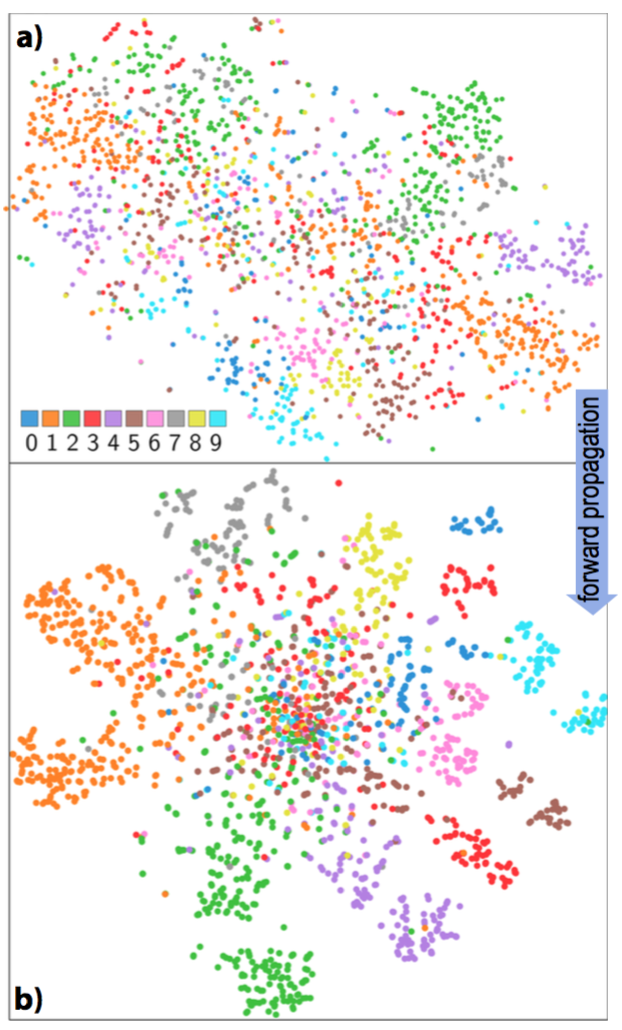
\includegraphics[width=0.5\textwidth]{figure/project-nn}
    \caption{Projection of the MLP hidden layer activations after training \cite{rauber2017hidden-activity}, SVHN test subset. a) First hidden layer. b) Last hidden layer.}
    \label{fig:project-nn}
\end{figure}

\subsection{Understanding}
The purposes of this task is to help researchers and developers better understand the characteristics and working mechanisms of different classifiers so that they can design a better one or choose a better one. The selection and design of the architecture of a classifier always require a strong expertise in machine learning, which needs cumulative experience of trial and error. For classifiers whose characteristics are still under studying (\eg, neural networks), such knowledge is even harder to achieve. Thus, most of the related work using visualization techniques for understanding classifiers focuses of neural networks. Considering the taxonomy of explanations, these visualizations mostly fall into model-aware global explanations, which provide a general sense of how a classifier behaves globally. Unlike pure explanation generation techniques, the visual analytics systems often embed extra information of the classifiers that boost understanding.
% Scientific understanding. Investigate the characteristic of the model.
These techniques can be roughly categorized into two: representation-based and component-based.

\textbf{Representation-based} methods visualize how a given set of instances is represented in the hidden layer or the final output of the classifier. As shown in \autoref{fig:project-nn}, Rauber \etal \cite{rauber2017hidden-activity} project the representations of a subset of instances in different layer, and verified that each layer of the network transform its input space to a more separable one. Unlike component-based methods, representation-based methods actually treat a model or a layer as a black box, and visualize how the representation space is transformed. This technique has been integrated in visual diagnostics systems such as ActiVis \cite{kahng2017activis} and DeepEyes \cite{pezzotti2017deep-eyes}. However, they are unable to analyze the detail information embedded in the classifiers.

\begin{figure}
    \centering
    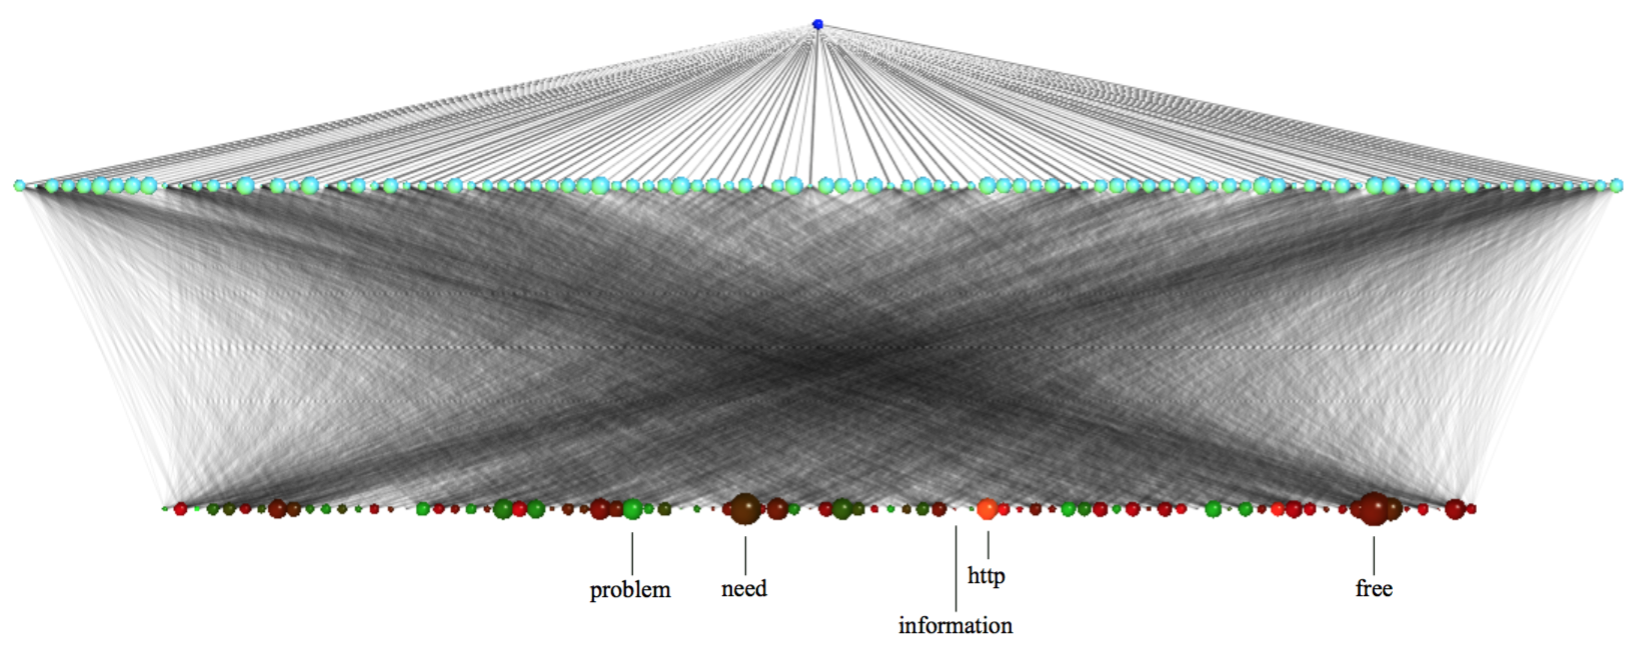
\includegraphics[width=1.0\textwidth]{figure/tzeng-nn}
    \caption{A spam classifier, where each input is a term in the email. The input data of the network is a subset of the spam in the training set \cite{tzeng2005visualize-nn}.}
    \label{fig:tzeng-nn}
\end{figure}

\begin{figure}
    \centering
    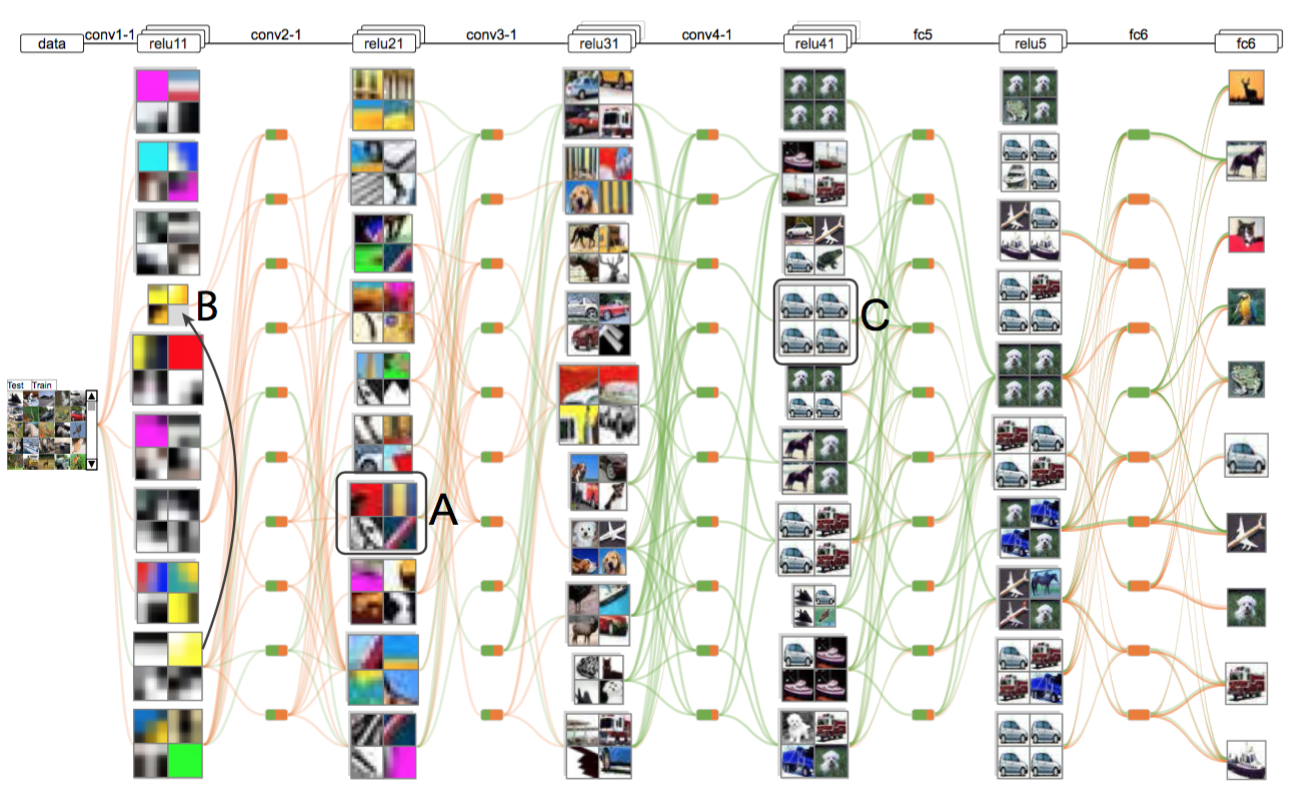
\includegraphics[width=1.0\textwidth]{figure/cnnvis}
    \caption{A visualization of a CNN with a large number of layers and neurons using neuron clustering and edge aggregation \cite{liu2017cnnvis}.}
    \label{fig:cnnvis}
\end{figure}

\textbf{Component-based} methods visualize the working mechanisms of specific components of a classifier. Tzeng and Ma directly visualize a multi-layer perceptron as a graph using the node-link layout. As shown in \autoref{fig:tzeng-nn}, though this visualization explained how important different term are for the neural network, it is visually cluttered and cannot reveal how neurons are combined to perform the classification. To provide more scalable visualization, Liu \etal develop the CNNVis \cite{liu2017cnnvis}, which use clustering and edge aggregation to provide a more compact visualization for CNNs. The representative image patch that activating each neuron clusters are also embedded in the visualization (see \autoref{fig:cnnvis}). There is also some work using visualization to understand RNNs. Karpathy \etal \cite{karpathy16rnn} visualize the value of a hidden unit along a sequence as a heatmap and find some hidden units have clear semantics. Strobelt \etal \cite{strobelt2017lstmvis} develop the LSTMVis based on parallel coordinates to identify dynamic patterns in the hidden state of an RNN. Ming \etal \cite{ming2017vast} develop the RNNVis, which is based on co-clustering and word clouds, and find that the hidden units can form semantics clusters from the text data.

These visualization techniques are proved to be able to provide insights and useful explanations of different classifiers. However, they are developed in a model-specific manner, which means they are difficult to generalize as common knowledge. There is also a lack of a unified process to visually analyze and understand a classifier, and a more rigorous measurement of how well a visualization helps explain the characteristics of a complex classifier.

\subsection{Diagnosis}

The diagnosis in the stage of model development mainly includes two parts: code diagnosis, and training diagnosis. Note that the diagnosis does not contribute to the explainability of a classifier directly. However, they can be thought to enhance the explainability of the code and training process of a classifier. Besides, the training difficulty varies as the architecture changes, which is also a part of characteristics of a classifier.

\begin{figure}
    \centering
    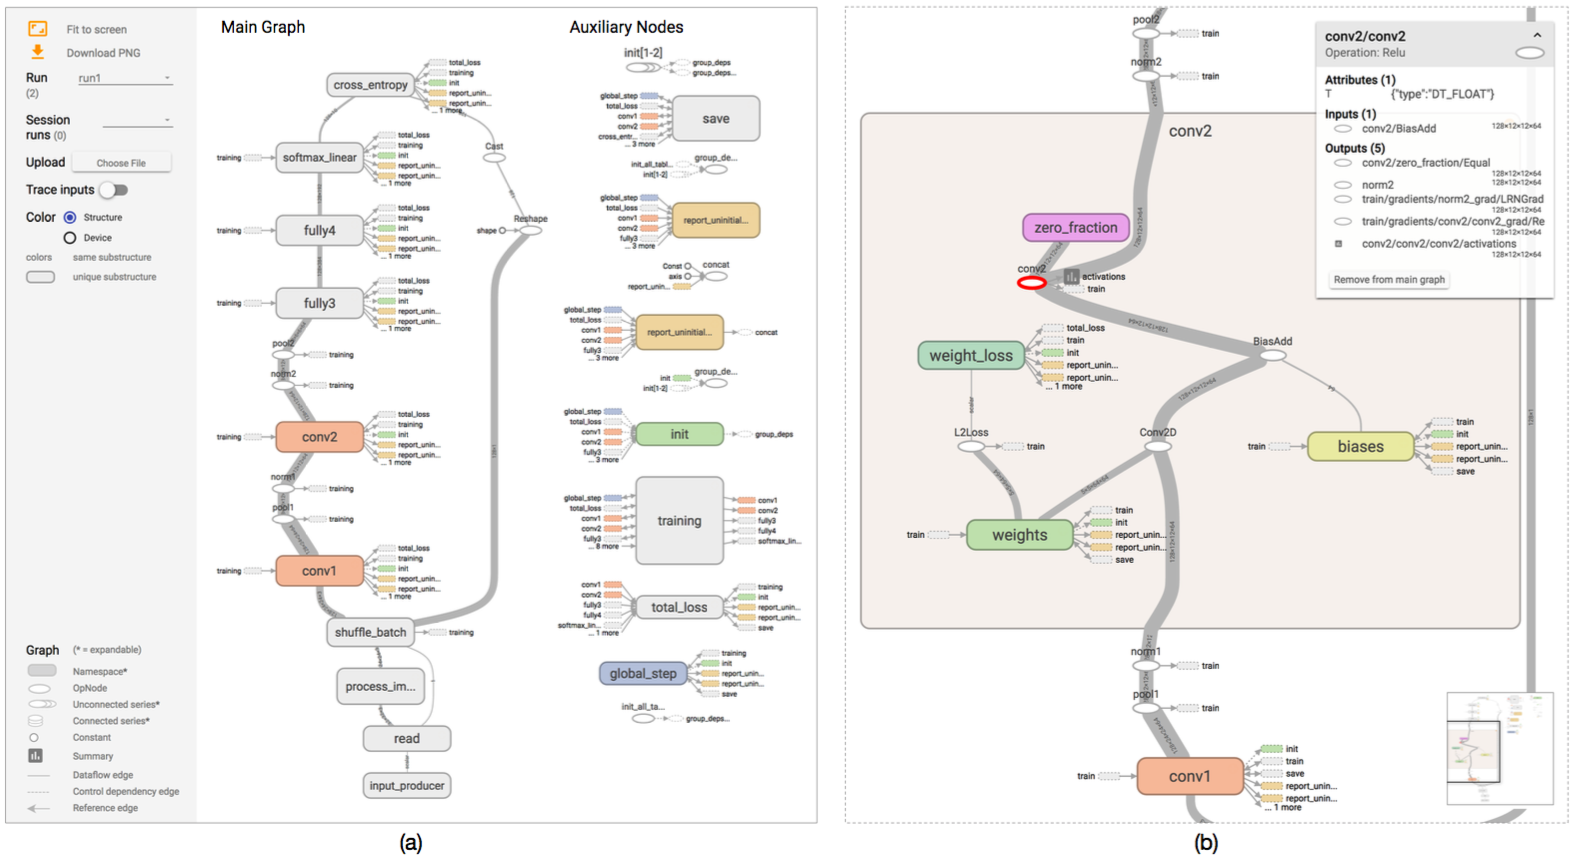
\includegraphics[width=1.0\textwidth]{figure/dataflow-graph}
    \caption{The TensorFlow Graph Visualizer shows a CNN image classifier \cite{wongsuphasawat2017dataflow}. (a) An overview displays a dataflow between groups of operations, with auxiliary nodes extracted to the side. (b) Expanding a group shows its nested structure.}
    \label{fig:dataflow-graph}
\end{figure}

\textbf{Code diagnosis.} Wongsuphasawat \etal \cite{wongsuphasawat2017dataflow} design and implemented a scalable graph layout for the data flow graph of any machine learning model and integrate the graph visualization in TensorFlow (see \autoref{fig:dataflow-graph}). The code defining the data flow graph can be automatically converted to a visualization, which helps developers validate the correctness of the code. A similar computation graph overview is proposed in the ActiVis, a visual exploration system for machine learning models developed by Kahng \etal \cite{kahng2017activis}.

\textbf{Training diagnosis.} There are also visual analytics systems developed to understand the training process of specific models. Unlike standard testing for software engineering, there is no accurate definition of the failure of a training. The failure of a training is a relative concepts. It is difficult to determine if a high loss is due to local optimum, the limitation of the model, or the quality of the dataset. Providing visual hints or indicator can help developers identify possible cause of failed training. The diagnosis of the training process is usually provided by sampling multiple snapshots during training. Liu \etal \cite{liu2017gan} develop the DGMTracker, which tracks the training process of the deep generative models (DGM) (\eg, generative adversarial model). They cache the training dynamics (\eg, activation changes) and visualize the training dynamics to help identify possible cause of a failed training. Pezzotti \etal \cite{pezzotti2017deep-eyes} proposed a progressive method that support the identification of layers that learn stable patterns and superfluous filters or layers. Visual analytics systems are also proved to be useful for tree boosting methods \cite{liu2017tree}. These visual analytics system are also model-specific and are difficult to generalize. There still needs further research in understanding the characteristics of the loss function to guide better the development of visualization techniques for training diagnosis.

\subsection{Assessment and Comparison} 

The purpose of evaluation is to determine if a trained classifier meets certain standards for deployment, and to select the best one among multiple classifiers. The evaluation is, to some extent, closely related to the training diagnostics. If a classifier fails the evaluation, then we will go back to adjust parameters for another training or refine its architecture. Visualization can also be used to assess and compare the performance of classifiers comprehensively (\eg, identify which classes the classifier is not good at). The visualization here also provide certain level of global explanations -- explaining a classifier using the statistics of its outputs of the test data. 

\begin{figure}[bt]
    \centering
    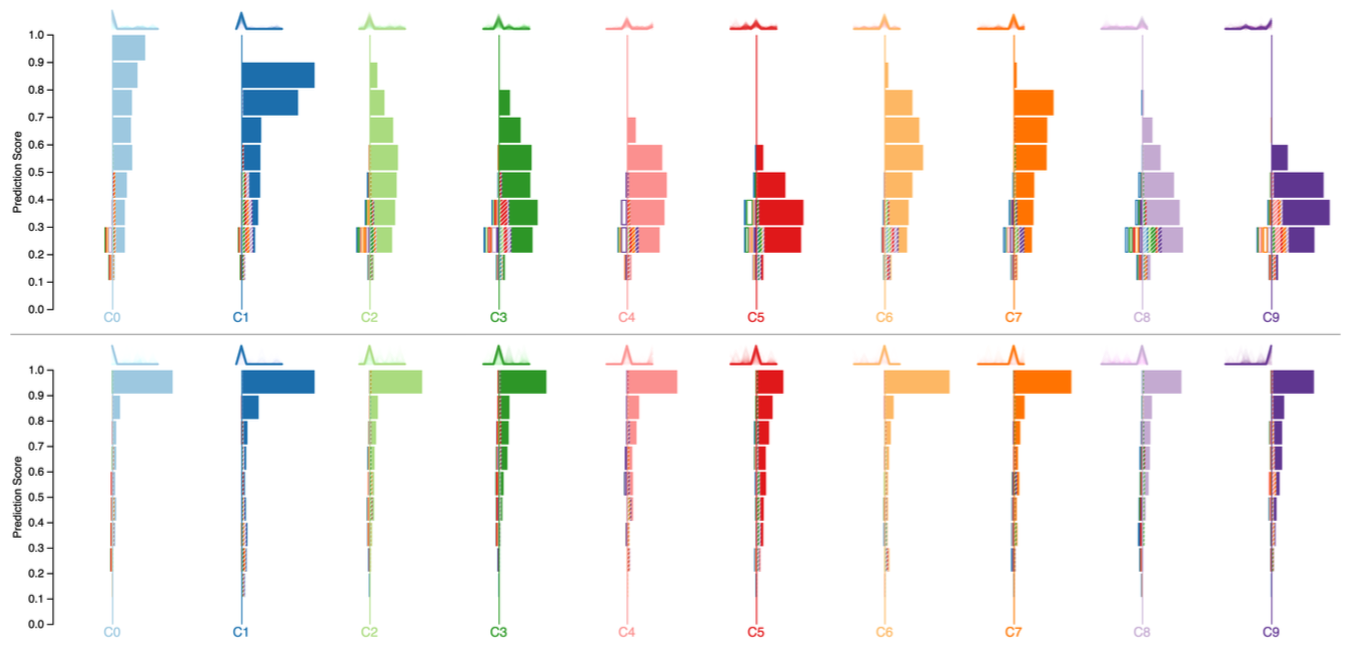
\includegraphics[width=1.0\textwidth]{figure/squares}
    \caption{Squares \cite{ren2017squares} displaying the performance of two classifier (top: random forest, bottom: SVM) trained on the MNIST dataset. They yield the same accuracy of 0.87 , but show vastly different score distributions.}
    \label{fig:squares}
\end{figure}

Amershi \etal \cite{amershi2015modeltracker} develop the ModelTracker to support the interactive performance analysis for binary classifier using stacked diagram. The ModelTracker combines the performance statistics and data inspection functions, which helps engineers evaluate the performance and identify problematic classifications at the same time.
Ren \etal extend it to the Squares \cite{ren2017squares}, which support the performance analysis for multi-class classifiers. As shown in \autoref{fig:squares}, the Squares is used to compare the performance of two classifiers, a random forest and an SVM, on the MNIST dataset. We can easily see that the SVM has much higher confidence than the random forest, though they have the same accuracy.
% \cite{muhlabacher2017treepod}

% There are plenty of opportunities to use visualization for evaluating and comparing classifiers. 

Currently, most evaluations only address accuracy and computation cost. As discussed in \autoref{sec-concepts}, we may need to meet other requirements such as fairness, robustness and explainability in certain applications. 
As discussed above, visualization can be used to enhance the explainability of a complex classifier. By explaining the reasoning of the classifier, we can identify possible discriminate classifications of the model. It is also possible to qualitatively evaluate the robustness of the classifier by verify if the classifier's reasoning matches that of a human or it is using unexpected reasoning. 

Except for the issues stated above, there are three general research issues for visualization in the model development stage. The first issue is the scalability of the visualization design. Many visualizations perform well in toy datasets such as MNIST. However, they will easily become overwhelming if the number of classes increases to a few hundreds. The second is the lack of consensus in the evaluation. The target of these visualization techniques is explaining and understanding, which is also subjective. It is difficult to design appropriate evaluation tasks for users to perform. The third is the need for a comprehensive toolkit that covers different procedures fluently. For example, TensorBoard\footnote{\url{https://github.com/tensorflow/tensorboard}} is a toolkit for visualizign and debugging machine learning models, which has been closely integrated in TensorFlow, but it is still at an early stage and has a limited set of functions.

\begin{figure}[bt]
    \centering
    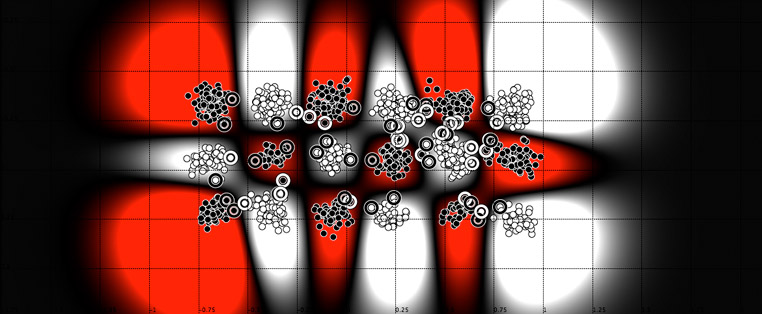
\includegraphics[width=1.0\textwidth]{figure/svm-rbf-points}
    \caption{A visualization from MLDemos, showing the decision space of a binary SVM classifier using RBF kernel. White and red denotes different classes, and black represents uncertainty.}
    \label{fig:mldemos}
\end{figure}

\subsection{Communication and Education}

Another related task, although not a necessary one in the model development stage, is the communicating and teaching of classification models. This task is related to the task of understanding. However, the focus of this task is not for a better understanding of the working mechanisms of a classifier, but for a better presentation of a classifier. 

% Visualization can directly help improve the explainability during the procedure of evaluation. There are other desirable properties except for a good accuracy, namely, fairness, robustness, and explainability. 

% Unquantifiable assessments, Fairness (e.g., discrimination), Vulnerability
With the growing complexity of model architectures, it often requires much effort to understand the composition and computation steps of a new classifier. It also requires a lot of work from the author to draw a diagram, which may neglect useful information for the readers. Netscope\footnote{\url{http://ethereon.github.io/netscope}} is a visualization tool that converts the code of a model written in Caffe\footnote{\url{http://caffe.berkeleyvision.org/}} to a node-link graph. Which helps quickly understand the topology of a model. However, the visualization will become too large if the model is complex (\eg, a CNN with a hundred layers), and it does not show extra information (\eg, optimizing method) about the model. TensorBoard utilizes the data flow graph visualization developed by Wongsuphasawat \cite{wongsuphasawat2017dataflow}, which is interactive and more scalable.

For new comers who want to learn, there will also be a large overhead to understand the computation of different components. Some visualizations have been developed to help people learn. Basilio Noris develops a visualization tool, MLDemos\footnote{\url{http://mldemos.epfl.ch/}} for understanding the behavior of various machine learning algorithms. As shown in \autoref{fig:mldemos}, MLDemos maps the output of a classifier using multiple colors back to the input space, and helps people learn the characteristics of different classifiers. Tensorflow Playground\footnote{\url{http://playground.tensorflow.org/}} is an interactive visualization, which helps people understand the behavior of a neural network, using similar techniques.


\section{Visualization for Operation}
The operation and management after deploying a classification system is an important stage of the whole life cycle, but  little attention has been paid to this stage. There are two common tasks that needs explainability: trust establishment and inspection.

\subsection{Trust Establishment}
The first challenge after the classifier has been deployed is how to establish users' trust in the machine.  Ribeiro \etal \cite{ribeiro2016kdd} have discussed the importance of a user's trust: if the user does not rust a model, he/she will not use it. If a user understand why the classifier predict class $A$ but not $B$, if he/she understand when the classifier performs well and when it is likely to fail, if he/she can figure out the possible reasons for a failure, he/she will trust the classifier. Thus, the foundation of trust is understanding, which can be achieved through explanation. Ribeiro \etal designed a inspiring solution for explanation, that is, locally approximate the complex classifier using an interpretable one, a linear classifier. Then the linear classifier is used to generate a local explanation (\eg, a list of words for a document classifier). Although this method introduces another classifier, whose error is not guaranteed, they showed that users indeed have more confident and trust in the classifier. Though explanation for trust establishment is promising, there are still unsolved issues. How to make sure the generated explanation is fidel to the model? How to evaluate whether the user has learned the correct message from the explanation? These should be addressed in future research.

\subsection{Monitoring}
After the end-users have established their trust in a classifier, they still needs a human-friendly interface to inspect or monitor the classifier. This need can be satisfied by providing faithful local explanations for specific predictions. The need for monitoring is not solely for preventing possible failure. For example, if we have developed a system for hospitals to detect early signs of lung cancer from CT scans, a good explanation not only helps the doctor correct possible false positives, but also provide the doctor extra information for deciding whether further examinations are needed. 



% \section{Evaluation}

% Review methods and standards of evaluating visualization.

% Address the problem of the lack of evaluation standards for visualization for explaianble classifiers.

% Proposed?

% 1. Fidelity. How visualization reflects the real model. (The relativeness and faithfulness of explanation)

% 2. Understandability. How easy the visualization is to be understood.

% \newpage

